% This code is a tweaked version of the script generated by GeoGebra (https://www.geogebra.org/)
% arara: latexmk: {options: [-pv]}
% arara: indent: {overwrite: yes, silent: yes, cruft: build}
\documentclass[tikz, border = 1pt]{standalone}

\usepackage{pgf, pgfplots}
\pgfplotsset{compat = 1.15}
\usepackage{mathrsfs}
\usetikzlibrary{arrows}

\definecolor{shadeofgreen}{HTML}{4daf4a}
\definecolor{shadeofred}{HTML}{e41a1c}
\definecolor{shadeofblue}{HTML}{377eb8}

\begin{document}
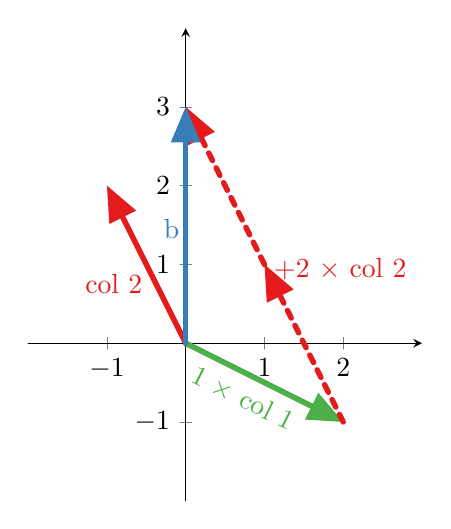
\begin{tikzpicture}[line cap = round, line join = round, >=triangle 45, x = 1cm, y = 1cm]
	\begin{axis}[
			x = 1cm, y = 1cm,
			axis lines = middle,
			xmin = -2,
			xmax = 3,
			ymin = -2,
			ymax = 4,
			xtick = {-1,..., 2},
			ytick = {-1,..., 3}
		]
		\clip(-2, -2) rectangle (3, 4);
		\draw [->, line width = 2pt, color = shadeofgreen] (0, 0) -- (2, -1);
		\draw [->, line width = 2pt, color = shadeofred] (0, 0) -- (-1, 2);
		\draw [->, line width = 2pt, dash pattern = on 3pt off 3pt, color = shadeofred] (2, -1) -- (1, 1);
		\draw [->, line width = 2pt, dash pattern = on 3pt off 3pt, color = shadeofred] (1, 1) -- (0, 3);
		\draw [->, line width = 2pt, color = shadeofblue] (0, 0) -- (0, 3);
		\draw [color = shadeofred] (1, 1.2) node[anchor = north west] {+2 \(\times\) col 2};
		\draw [color = shadeofred] (-1.4, 1) node[anchor = north west] {col 2};
		\draw [color = shadeofgreen] (0.1, -0.1) node[rotate = -26.6, anchor = north west] {1 \(\times\) col 1};
		\draw [color = shadeofblue] (-0.4, 1.7) node[anchor = north west] {b};
	\end{axis}
\end{tikzpicture}
\end{document}
